\documentclass{../../class}

\title{4231 Homework 4}
\author{Eumin Hong (eh2890)}
\date{\today}

\begin{document}
\maketitle

\lhead{4231 Homework 4}
\rhead{Eumin Hong (eh2890)}

\tcbset{colback=blue!5, colframe=blue!75!black}

\section*{Problem 1}
\begin{tcolorbox}
    Problem 15.3 on Page 405: Bitonic euclidean traveling-salesman problem.
\end{tcolorbox}
\section*{15.3}
In the \textbf{\textit{euclidean traveling-salesman problem}}, we are given a set of $n$ points in the plane, and we wish to find the shortest closed tour that connects all $n$ points. Figure \ref{fig:15-11.png}(a) shows the solution to a $7$-point problem. The general problem is NP-hard, and its solution is therefore believed to require more than polynomial time (see Chapter 34).

J. L. Bentley has suggested that we simplify the problem by restricting our attention to \textbf{\textit{bitonic tours}}, that is, tours that start at the leftmost point, go strictly rightward to the rightmost point, and then go strictly leftward back to the starting point. Figure \ref{fig:15-11.png}(b) shows the shortest bitonic tour of the same 7 points. In this case, a polynomial-time algorithm is possible.

Describe an $O(n^2)$-time algorithm for determining an optimal bitonic tour. You may assume that no two points have the same $x$-coordinate and that all operations on real numbers take unit time. (\textit{Hint}: Scan left to right, maintaining optimal possibilities for the two parts of the tour.)

\begin{figure}[H]
    \centering
    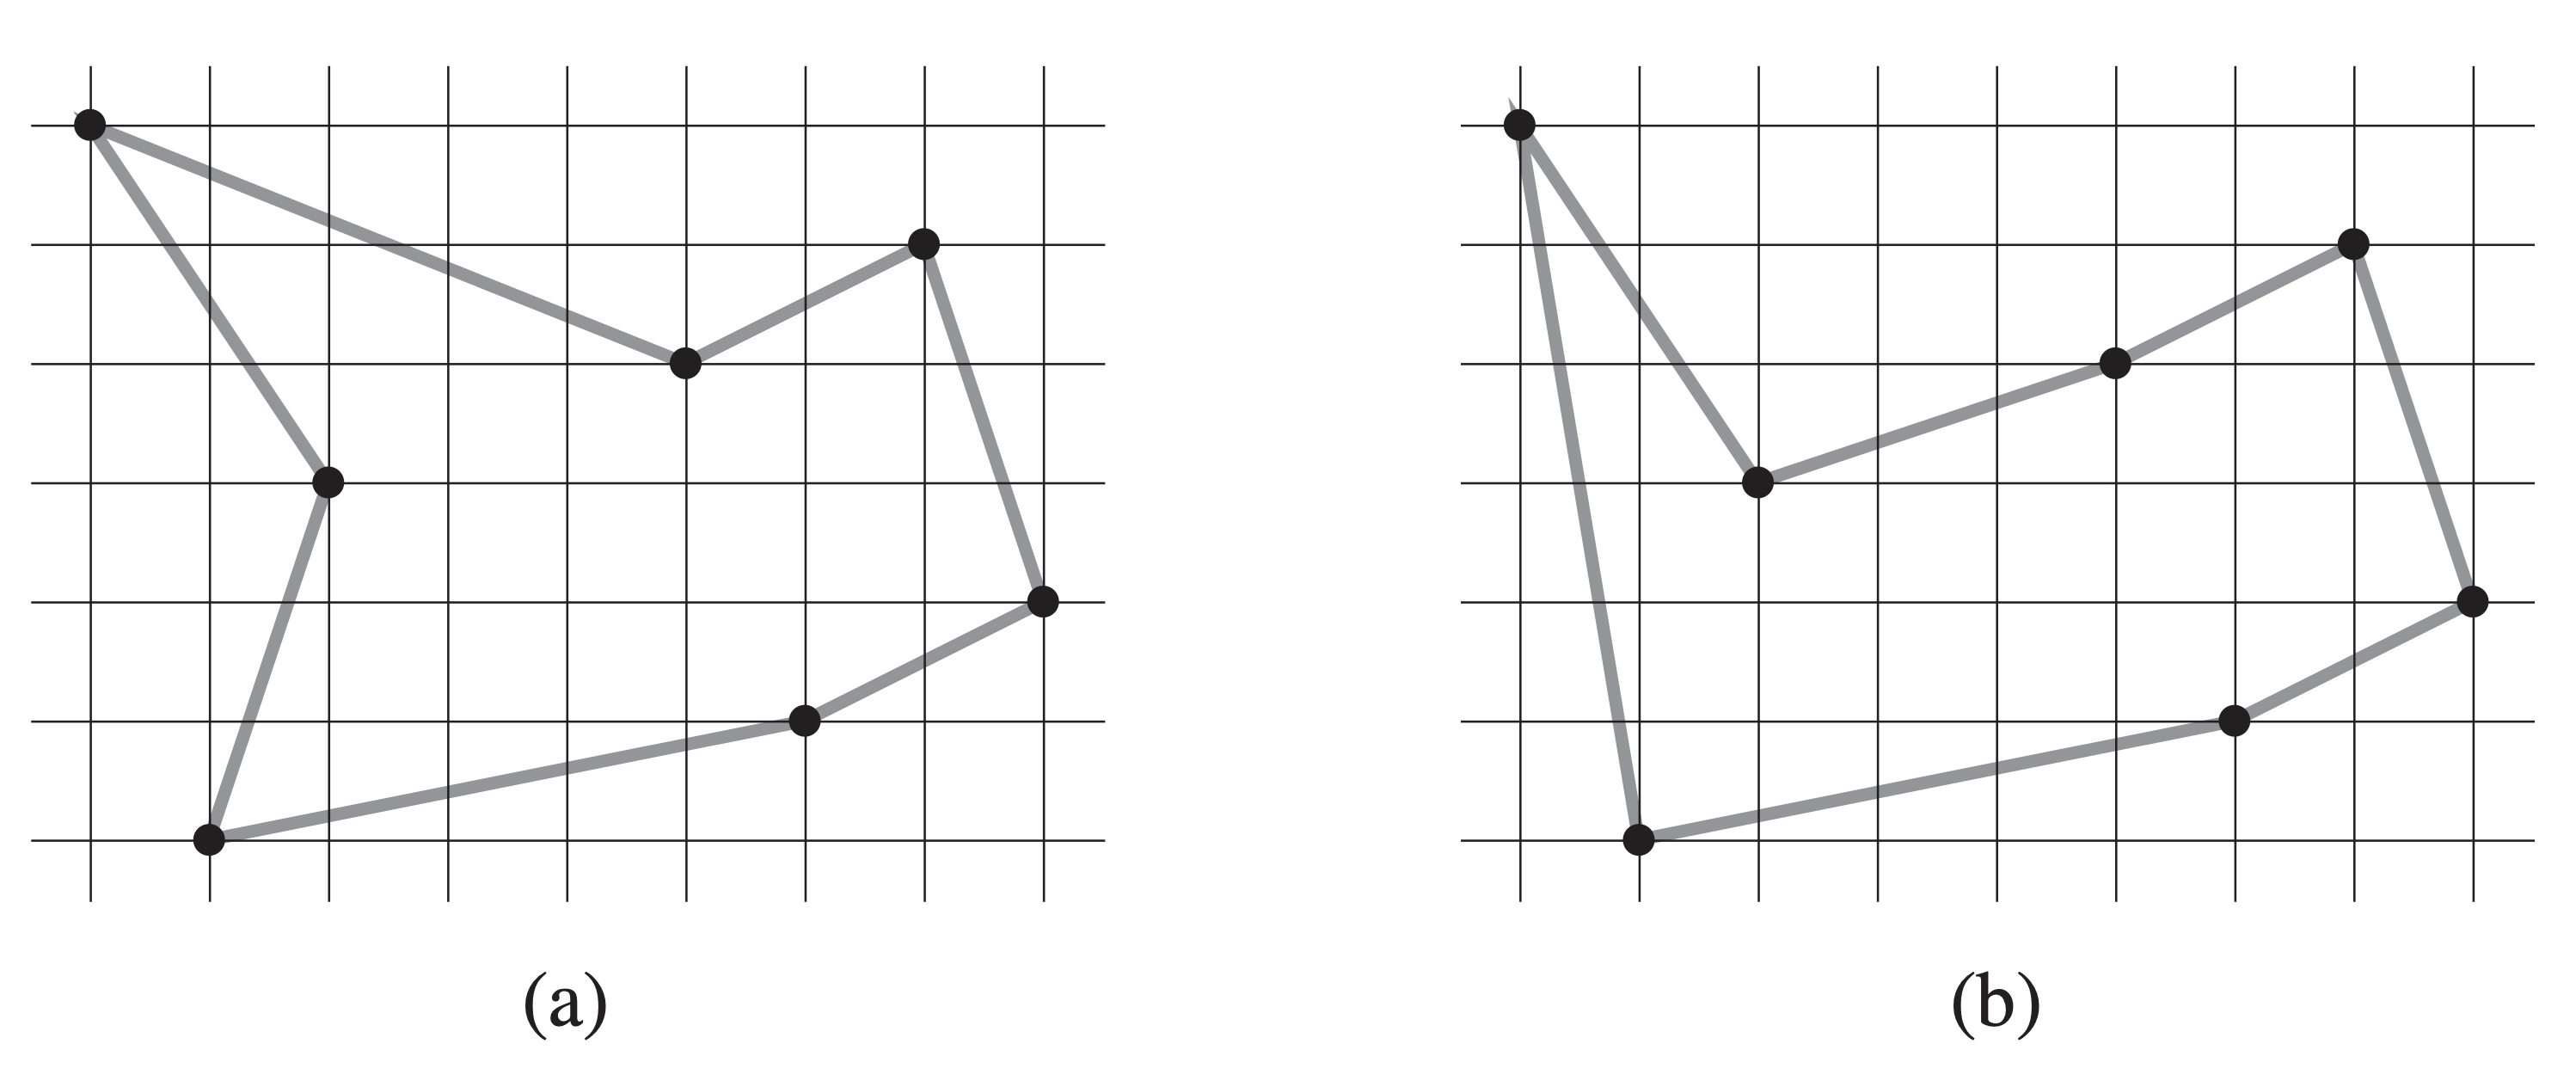
\includegraphics[width = 10cm]{img/15-11.png}
    \caption{Seven points in the plane, shown on a unit grid. \textbf{(a)} The shortest closed tour, with length approximately $24.89$. This tour is not bitonic. \textbf{(b)} The shortest bitonic tour for the same set of points. Its length is approximately $25.58$.}
    \label{fig:15-11.png}
\end{figure}

\newpage
\section*{Problem 2}
\begin{tcolorbox}
    Exercise 15.1-2 on Page 370: Counterexample.
\end{tcolorbox}
\subsection*{15.1-2}
Show, by means of a counterexample, that the following \enquote{greedy}
strategy does not always determine an optimal way to cut rods. Define the density of a rod of length $i$ to be $p_i/i$, that is, its value per inch. The greedy strategy for a rod of length $n$ cuts off a first piece of length $i$, where $1 \leq i \leq n$, having maximum density. It then continues by applying the greedy strategy to the remaining piece of length $n - i$.

\newpage
\section*{Problem 3}
\begin{tcolorbox}
    Problem 17-2 on Page 473 (Skip c): Making binary search dynamic.
\end{tcolorbox}
\subsection*{17-2}
Binary search of a sorted array takes logarithmic search time, but the time to insert a new element is linear in the size of the array. We can improve the time for insertion by keeping several sorted arrays.

Specifically, suppose that we wish to support \textsc{Search} and \textsc{Insert} on a set of $n$ elements. Let $k = \lceil \lg{(n+1)} \rceil $, and let the binary representation of $n$ be $\langle n_{k-1}, n_{k-2}, \dots, n_0 \rangle $. We have $k$ sorted arrays $A_0, A_1, \dots,$ $A_{k-1}$, where for $i = 0, 1, \dots, k-1$, the length of array $A_i$ is $2^i$. Each array is either full or empty, depending on whether $n_i = 1$ or $n_i = 0$, respectively. The total number of elements held in all $k$ arrays is therefore $\sum_{i=0}^{k-1} n_i2^i = n$. Although each individual array is sorted, elements in different arrays bear no particular relationship to each other.
\begin{enumerate}[\textbf{\textit{\alph*.}}]
    \item Describe how to perform the \textsc{Search} operation for this data structure. Analyze its worst-case running time.
    \item Describe how to perform the \textsc{Insert} operation. Analyze its worst-case and amortized running times.
\end{enumerate}

\newpage
\section*{Problem 4}
\begin{tcolorbox}
    Problem 17-3 on Page 473: Amortized weight-balanced trees.
\end{tcolorbox}
\subsection*{17-3}
Consider an ordinary binary search tree augmented by adding to each node $x$ the attribute $x.size$ giving the number of keys stored in the subtree rooted at $x$. Let $\alpha $ be a constant in the range $1/2 \leq \alpha < 1$. We say that a given node $x$ is $\mathbb{\alpha}$\textbf{-balanced} if $x.left.size \leq \alpha \cdot x.size$ and $x.right.size \leq \alpha \cdot x.size$. The following amortized approach to maintaining weight-balanced trees was suggested by G. Varghese.
\begin{enumerate}[\textbf{\textit{\alph*.}}]
    \item A $1/2$-balanced tree is, in a sense, as balanced as it can be. Given a node $x$ in an arbitrary binary search tree, show how to rebuild the subtree rooted at $x$ so that it becomes $1/2$-balanced. Your algorithm should run in time $\Theta (x.size)$, and it can use $O(x.size)$ auxiliary storage.
    \item Show that performing a search in an $n$-node $\alpha$-balanced binary search tree takes $O(\lg{n})$ worst-case time.

    For the remainder of this problem, assume that the constant $\alpha$ is strictly greater than $1/2$. Suppose that we implemented \textsc{Insert} and \textsc{Delete} as usual for an $n$-node binary search tree, except that after every such operation, if any node in the tree is no longer $\alpha$-balanced, then we \enquote{rebuild} the subtree rooted at the highest such node in the tree so that it becomes $1/2$-balanced.

    We shall analyze this reuilding scheme using the potential method. For a node $x$ in a binary search tree $T$, we define
    \begin{gather*}
        \Delta(x) = |x.left.size - x.right.size|,
    \end{gather*}
    and we define the potential of $T$ as
    \begin{gather*}
        \Phi(T) = c \sum_{x\in T: \Delta(x) \geq 2} \Delta(x), 
    \end{gather*}
    where $c$ is a sufficiently large constant that depends on $\alpha$.
    \item Argue that any binary search tree has nonnegative potential and that a $1/2$-balanced tree has potential $0$.
    \item Suppose that $m$ units of potential can pay for rebuilding an $m$-node subtree. How large must $c$ be in terms of $\alpha$ in order for it to take $O(1)$ amortized time to rebuild a subtree that is not $\alpha$-balanced?
    \item Show that inserting a node into or deleting a node from an $n$-node $\alpha$-balanced tree costs $O(\lg{n)}$ amortized time.
\end{enumerate}

\newpage
\section*{Problem 5}
\begin{tcolorbox}
    Exercise 22.2-6 and 22.2-7 on Page 602.
\end{tcolorbox}
\subsection*{22.2-6}
Give an example of a directed graph $G = (V, E)$, a source vertex $s\in V$, and a set of tree edges $E_\pi \subseteq E$ such that for each vertex $v\in V$, the unique simple path in the graph $(V, E_\pi)$ from $s$ to $v$ is shortest path in $G$, yet the set of edges $E_\pi$ cannot be produced by running BFS on $G$, no matter how the vertices are ordered in each adjacency list.

\subsection*{22.2-7}
There are two types of professional wrestlers: \enquote{babyfaces} (\enquote{good guys}) and \enquote{heels} (\enquote{bad guys}). Between any pair of professional wrestlers, there may or may not be a rivalry. Suppose we have $n$ professional wrestlers and we have a list of $r$ pairs of wrestlers for which there are rivalries. Give an $O(n+r)$-time algorithm that determines whether it is possible to designate some of the wrestlers as babyfaces and the remainder as heels such that each rivalry is between a babyface and a heel. If it is possible to perform such a designation, your algorithm should produce it.

\end{document}
